\section{Problem Formulation and SkillAudit}

\subsection{Problem Formulation}

Let a paper $P$ describe a bounded procedure to be reused by an LLM agent. An upstream extraction system produces a \emph{full specification} $F$, and an upstream reducer produces a shorter \emph{candidate specification} $S$. We do not assume that $F$ is complete or that $S$ is faithful. Given a task $t$ and an evaluation boundary $\Omega$, our question is whether $S$ can substitute for $F$ without making the task solvable from the task statement alone. We therefore compare three artifact conditions: $B$, a no-specification baseline; $F$, the full specification; and $S$, the simplified candidate.

The paper procedure is represented by source-addressed atoms $A=\{a_1,\ldots,a_K\}$ and a directed acyclic dependency graph $G=(A,E)$. Each atom is
\begin{equation}
a_i=(\mathrm{id}_i,\ell_i,u_i,r_i,D_i),
\label{eq:atom}
\end{equation}
where $\ell_i$ is an exact locator in the identified paper, $u_i$ is an executable instruction, $r_i$ records its procedural role, and $D_i$ contains the identifiers of its direct prerequisites. A candidate atom set $A_S\subsetneq A$ is admissible for evaluation only if it is nonempty, acyclic, and dependency closed: $D_i\subseteq\{\mathrm{id}_j:a_j\in A_S\}$ for every $a_i\in A_S$. A deterministic renderer $R$ then produces $F=R(A)$ and $S=R(A_S)$. This representation proves which source content was retained or removed; it does not prove that either artifact is behaviorally sufficient.

For each registered block $r\in\{1,\ldots,n\}$ and condition $C\in\{B,F,S\}$, an agent receives the same task, starter workspace, tools, public test, action budget, and private scorer. Only the assigned artifact changes. The resulting terminal row contains a validity bit $v_{C,r}$, a hard-contract bit $h_{C,r}$, a patch-present bit $p_{C,r}$, and a private score $q_{C,r}\in[0,1]$. With a prespecified score threshold $\tau$, operational success is
\begin{equation}
z_{C,r}=\mathbb{1}\!\left[v_{C,r}=1\land h_{C,r}=1\land p_{C,r}=1\land q_{C,r}\ge\tau\right].
\label{eq:success}
\end{equation}
The block count $k_C=\sum_{r=1}^{n}z_{C,r}$ is descriptive evidence for this finite schedule, not an estimate of a universal success probability.

\begin{figure*}[t]
\centering
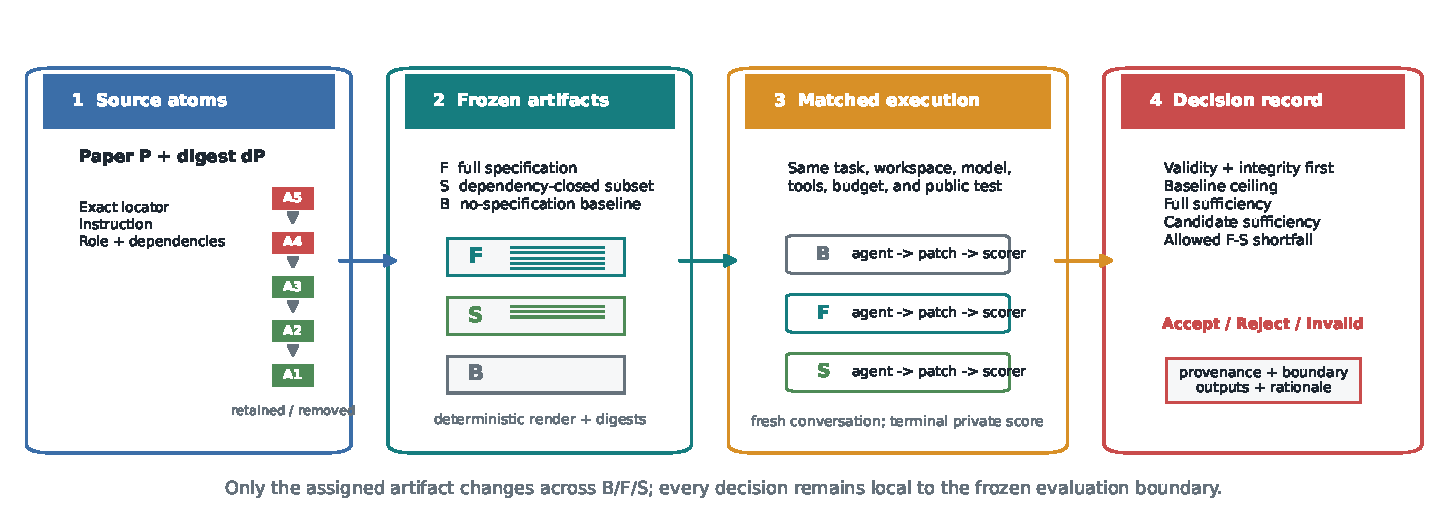
\includegraphics[width=\textwidth]{images/skillaudit_overview.pdf}
\caption{End-to-end SkillAudit protocol. A paper is decomposed into source-addressed atoms and explicit dependencies; green atoms are retained by the candidate and red atoms are removed. The full specification $F$, simplified candidate $S$, and no-specification baseline $B$ are frozen and run under matched task and execution conditions. Validity and integrity are checked before the finite-schedule gate produces \textsc{Accept}, \textsc{Reject}, or \textsc{Invalid}. The evidence record binds provenance, the frozen boundary, terminal outputs, and the decision rationale.}
\label{fig:overview}
\end{figure*}

\subsection{SkillAudit Overview}

Figure~\ref{fig:overview} shows the complete information flow. SkillAudit is a post-compression validator rather than a reducer: it accepts candidates generated by a heuristic, learned, or interactive upstream method, but never edits a candidate after held-out evaluation begins. The protocol first verifies the source map and dependency closure, then freezes the artifacts and experimental boundary, executes matched $B/F/S$ blocks, validates every terminal row, applies a prespecified decision rule, and emits an evidence record. Algorithm~\ref{alg:skillaudit} states the same procedure operationally.

\begin{algorithm}[t]
\caption{SkillAudit for one fixed candidate}
\label{alg:skillaudit}
\begin{algorithmic}[1]
\REQUIRE Paper $P$, atoms $(A,G)$, candidate $A_S$, task $t$, boundary $\Omega$
\STATE Verify paper identity, source locators, DAG validity, and closure of $A_S$
\STATE Render and freeze $F=R(A)$, $S=R(A_S)$, and baseline $B$
\FOR{each registered block $r$ and condition $C\in\{B,F,S\}$}
    \STATE Execute a fresh agent session and retain the complete terminal output
    \STATE Validate digests, submission, patch, scorer, and hard task contract
\ENDFOR
\IF{the registered schedule or an integrity check is incomplete}
    \STATE $\delta\leftarrow\textsc{Invalid}$
\ELSE
    \STATE Compute $k_B,k_F,k_S$ and apply the frozen acceptance rule
    \STATE $\delta\leftarrow\textsc{Accept}$ if all fields pass; otherwise $\textsc{Reject}$
\ENDIF
\STATE Emit source links, $\Omega$, terminal outputs, field-level checks, and $\delta$
\end{algorithmic}
\end{algorithm}

\subsection{Source-Addressed Candidate Construction}

The atom registry is constructed from quoted paper passages. Exact document digests and page, line, or byte spans make the mapping inspectable, while $r_i$ distinguishes operations, parameters, guards, ordering constraints, and output contracts. Dependencies are recorded separately from prose order because a prerequisite may be stated in another paragraph, caption, or equation. The closure auditor rejects unknown identifiers, graph cycles, a non-strict subset, or a retained atom whose prerequisite is absent. Rendering uses a fixed topological order with atom-identifier tie breaking, so the same registry produces byte-identical artifacts.

The candidate boundary remains explicit. For example, if $a_4$ implements a solver and depends on preprocessing atoms $a_1$--$a_3$, retaining $a_4$ while removing $a_2$ is a structural failure before any model call. Removing $a_4$ while retaining $a_1$--$a_3$ can be structurally valid but behaviorally insufficient. This separation prevents a dependency check from being overinterpreted as a reproduction guarantee. It also permits failure analysis to point back from a rejected candidate to the exact source units that were omitted.

\subsection{Frozen Evaluation Boundary}

The evaluation boundary binds every factor that may change the interpretation of a comparison:
\begin{equation}
\Omega=(P,A,G,F,S,t,W,M,T,U,Q,\sigma,\tau,\gamma),
\label{eq:boundary}
\end{equation}
where $W$ is the starter workspace, $M$ the model and decoding configuration, $T$ the tool interface, $U$ the action budget, $Q$ the public and private tests plus scorer, $\sigma$ the blocked condition schedule, $\tau$ the operational-success threshold, and $\gamma$ the acceptance thresholds. Digests bind the concrete files associated with these symbols. The block order is balanced when the schedule permits, and every condition starts from an isolated workspace and fresh conversation.

Public tests are visible development feedback: the agent may run them before submission. The private scorer is terminal and one-way. Once the agent submits a patch, the patch is frozen, the private cases are executed once, and no private result is returned to the agent. This boundary limits direct adaptation to hidden cases while preserving a realistic development loop. Case-generation seeds, registry assignments, and condition order are recorded. When a provider does not expose an enforceable sampling seed, the record explicitly distinguishes deterministic orchestration from nondeterministic model execution.

\subsection{Validity Before Performance}

SkillAudit separates execution validity from task failure. A valid scored failure includes a submitted patch that violates the hard output contract or falls below $\tau$; it contributes $z_{C,r}=0$ to the registered denominator. A row is invalid when the registered request was not executed as specified, an expected output or digest is missing, the scorer did not complete, or the provider/model was unavailable after the retry policy. Malformed or empty submissions are recorded as their own terminal category and are interpreted according to the frozen row-validity rule. This taxonomy prevents network, wrapper, serialization, and scoring defects from being silently counted as evidence that a skill is insufficient.

Let $V=1$ only when all required rows and schedule-level integrity checks are complete. With a baseline ceiling $b_{\max}$, minimum full and candidate counts $f_{\min}$ and $s_{\min}$, and maximum allowed shortfall $\epsilon$, the decision is
\begin{equation}
\delta_{t,\Omega}(S)=
\begin{cases}
\textsc{Invalid}, & V=0,\\
\textsc{Accept}, & \begin{aligned}
&V=1,\ k_B\le b_{\max},\ k_F\ge f_{\min},\\[-2pt]
&k_S\ge s_{\min},\ k_F-k_S\le\epsilon,
\end{aligned}\\
\textsc{Reject}, & \text{otherwise.}
\end{cases}
\label{eq:decision}
\end{equation}
The baseline ceiling checks that the task is not already easy without a specification. Full sufficiency checks that the reference artifact and evaluation package can support the task. Candidate sufficiency and the $F-S$ shortfall test the substitution claim. A rejection is local: it withholds permission to substitute under $(t,\Omega)$ and does not declare the candidate semantically wrong for every task or model.

\subsection{Auditable Evidence Record}

The output is not only a label. SkillAudit emits
\begin{equation}
\mathcal{E}=(d_P,d_A,d_F,d_S,d_{\Omega},\mathcal{O},\mathcal{C},\delta,\rho),
\label{eq:evidence}
\end{equation}
where the $d$ terms identify the paper, atom registry, artifacts, and boundary; $\mathcal{O}$ is the immutable set of requests, trajectories, patches, scores, and transport attempts; $\mathcal{C}$ contains field-level validity and acceptance checks; and $\rho$ is a human-readable rationale. Consequently, an accepted candidate can be distributed with the exact task and evidence that support its use, while a rejected or invalid candidate carries a diagnosis rather than an unqualified failure label.
